\section{Solution comparison}
In this section we will look at the current solution at \siemens and our own solution to the problem, to see how they compare in different areas.

\subsection{Resulting schedule comparison}

Our system creates a work schedule that upholds all the union agreements, meaning that human mistakes are not possible as in the schedule currently made by \siemens. We have also made a grading system that would be unbiased regarding what days to add or remove, unless humans intervene through the criteria system. Our schedule however, does lack some of the visual attributes that the standard schedule has, when unedited. 

\begin{figure}[ht!]
    \centering
    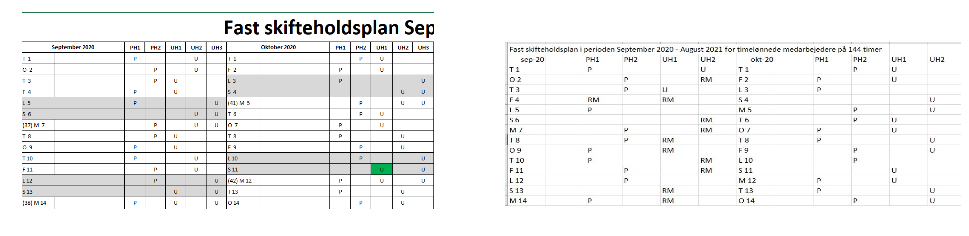
\includegraphics[width=\textwidth]{media/Comparison of Schedules.png}
    \caption{The left is the desired schedule, and the right is our unedited schedule}
    \label{fig:Our_Table}
\end{figure}

As shown above, the desired work schedule has color-coding, borderlines and a larger title. It is not possible through a .csv file to add colour and text-size to the schedule. That is why the person working with creating the schedule still needs to manually insert the different visual effects.

Our schedule also has a tendency to remove shifts earlier in the year, because it currently takes the first shift with highest priority, so the first SH-day would be removed, where a manual worker more likely would spread out the shifts removed. 

\subsection{Time comparison}
At last we want to show if our solution will actually be better than the system \siemens currently has. Our solution currently takes less than a second to read the input-file and write the output file. If we take into consideration that a user must also add the different visuals that the workers expect, that, in our own tests, took approximately 9 minutes, which was the time we used in testing. This means that the whole process of creating the work schedule can be done in less than 10 minutes.

Compared to the method that \siemens is currently using that takes about four uninterrupted hours, this method is much faster. It should also be noted that the person who is currently in charge of scheduling is very experienced in this area and would most likely be much faster than an inexperienced employee. Furthermore, this method does not mean you have to know the different requirements of making a schedule, the program does it for you. This means that the learning process of making a work schedule is also shortened to a few minutes.

So we can conclude that our solution is a viable improvement to the system currently used at \siemens, as it is both executed much faster and the time learned to master our system will be significantly lower, and much less prone to making mistakes, as it will create the work schedule reliably, and only need human input to make it look more appealing, and to specify different aspects if the work-schedule is not accepted.

